\section{Solutions}
\subsection{Choice of Input}

<<<<<<< HEAD
To gain useful information from the camera, which was positioned next to the arm on the table, classic image processing was used to extract features from the camera frames. An efficient algorithm for extracting the center points of the hand and the target object was implemented and an example of a processed image, with respect to its original image, is shown in figure \ref{fig:processed_pic}.Due to the hardly limited scope of the camera the extracted informations could unfortunately not be used to improve our results.
=======
To gain useful information from the camera which was positioned next to the arm on the table classic image processing was used to extract features from the camera frames. An efficient algorithm for extracting the center points of the hand and the target object was implemented and an example of a processed image with respect to its original image is shown in figure \ref{processed_pic}. Due to the limited scope of the camera the extracted informations could unfortunately not be used to improve our results.\\
>>>>>>> 32d0de4ac4ce6b832b85dd8c8628ff556a18aad4

\begin{figure}[H]
	\centering
	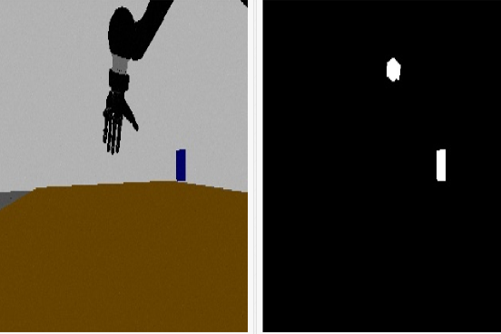
\includegraphics[width=2.2in]{img/image_processing.png}
	\DeclareGraphicsExtensions.
	\caption{Original image (left) and processed image with extracted hand and target (right)}
	\label{fig:processed_pic}
\end{figure}

<<<<<<< HEAD
Thus, only the center object was directly read from the system and was used all the time as input to the spiking neural network. The high changing rate of the input were one reason why the results were hardly unreproducible. To fix this problem the update rate of the input was decreased and the values itself were rounded to the second decimal position, what led to slightly better reproducibility. 
=======
Thus, only the center object was directly read from the system and was used all the time as input to the spiking neural network. The high changing rate of the input were one of the reasons why the results were hardly reproducible. To fix this problem the update rate of for the input was decreased and the values itself were casted to the second decimal position what led to slightly better reproducibility. 
>>>>>>> 32d0de4ac4ce6b832b85dd8c8628ff556a18aad4

\subsection{Learning Approaches}
%Hier sollte erwähnt werden wieso wir Evolutionär Algorithmen verwenden und keine klassischen Neuronalen Netze
%Bild mit Evolutionärer Algrotithmus allgemein, falls das noch nicht in Part 1 steht
Current methods for training spiking neural networks are often based on plasticity either spike-timing-dependent (STDP), rate-based, reward based or structural or are based on evolutionary algorithms. %hier sollte noch irgendwas dazwischen gerade halt keine idee :D
 For our purpose we chose an evolutionary approach. The basic idea behind an evolutionary or genetic algorithm is based upon biological evolution where the fitness of an individual decides if it survives and generates offspring. Given an initial population these algorithms are usually divided into 3 steps, as shown in Fig. \ref{evo_base}. 1) Evaluate the fitness of each individual given a fitness function f(). In our case this function is the distance achieved by running the experiment in the simulation. 2) Select the best-fit individuals for reproduction. 3) Breed and mutate individuals to generate offsprings.

\begin{figure}[H]
	\centering
	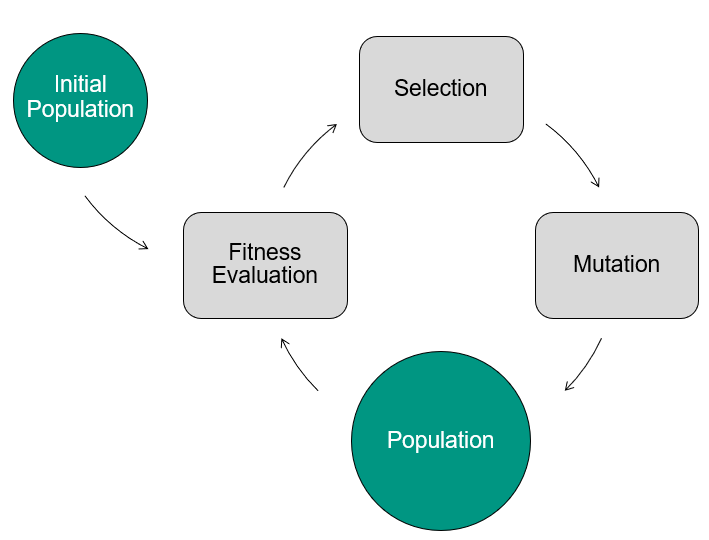
\includegraphics[width=2.2in]{img/evo_base.png}
	\DeclareGraphicsExtensions.
	\caption{General scheme of an evolutionary algorithm}
	\label{evo_base}
\end{figure}

\subsubsection{Evolutionary Strategy 1}


<<<<<<< HEAD
To verify the correct and efficient implementation of our algorithms, an evaluation function was written to reduce simulation effort in the Neurorobotics platform. The evaluation function makes sure that the search for maxima in the feature space will be successful. The test scenario can be seen as a hill climbing problem with the distance function as the reward which is returned for every weight batch that is passed to it. The exemplary chosen function space is shown in blue and the best return values of our algorithm in red in figure \ref{fig:test_function}. For testing purposes the feature space was reduced to 2 weights and is increased to the number of output neurons during the test phase.
Like it's represented in figure \ref{fig:test_function}, once a good starting point is found the algorithm starts varying the weights to increase the reward. 
=======
To verify the correct and efficient implementation of our algorithms an evaluation function was written to reduce simulation effort in the Neurorobotics platform. The evaluation function makes sure that the search for maxima in the feature space will be successful. The test scenario can be seen as a hill climbing problem with the distance function as the reward which is returned for every weight batch that is passed to it. The exemplary chosen function space is shown in blue and the best return values of our algorithm in red in figure \ref{fig:test_function}. For testing purposes the feature space was reduced to 2 weights and is increased to the number of output neurons during the test phase.
As you can see in figure \ref{fig:test_function}, once a good starting point is found the algorithm starts varying the weights to increase the reward. 
>>>>>>> 32d0de4ac4ce6b832b85dd8c8628ff556a18aad4

\begin{figure}[H]
	\centering
	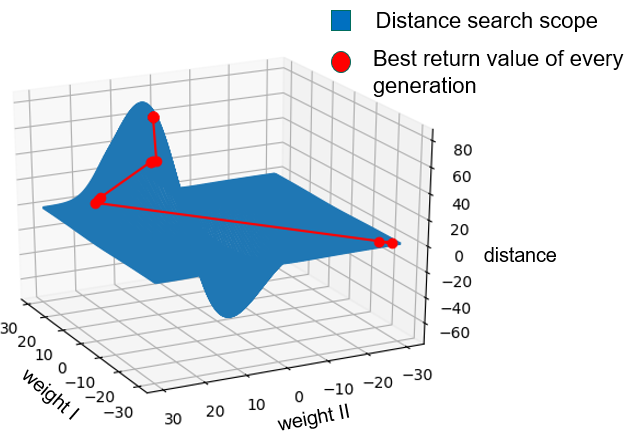
\includegraphics[width=3.3in]{img/test_function.png}
	\DeclareGraphicsExtensions.
	\caption{Output plot of the test function with the evolutionary algorithm 1}
	\label{fig:test_function}
\end{figure}

The overall idea behind the final algorithm for our first evolutionary strategy itself can be seen in figure \ref{fig:evo_strat_1}. The basic strategy to make sure that the algorithm converges as fast as possible is to change the weights not only randomly but in the direction where the highest improvement is expected. Hence, the set of weights at iteration k is expected to increase the reward if the difference to the last reward is positive. In this case the normalized distance from the weights $w_k$  at the current iteration to $w_{k-1}$ from the last iteration is added to the weights of the next iteration and otherwise the distance is subtracted. To add a certain randomness to the algorithm, a merge of different sets of weights every 10th epoch is implemented by fusing a random amount of weights in several dimensions. This randomness was added in order to avoid to get stuck in local maxima or in case that high potentially areas in the feature space are too far away from the current position of the weights. After every generation of weights, the learning rate is decreased to scan the feature space more precisely for the best result. 
The results of the presented approach are discussed in section\ref{sec:results}.

\begin{figure}[H]
	\centering
	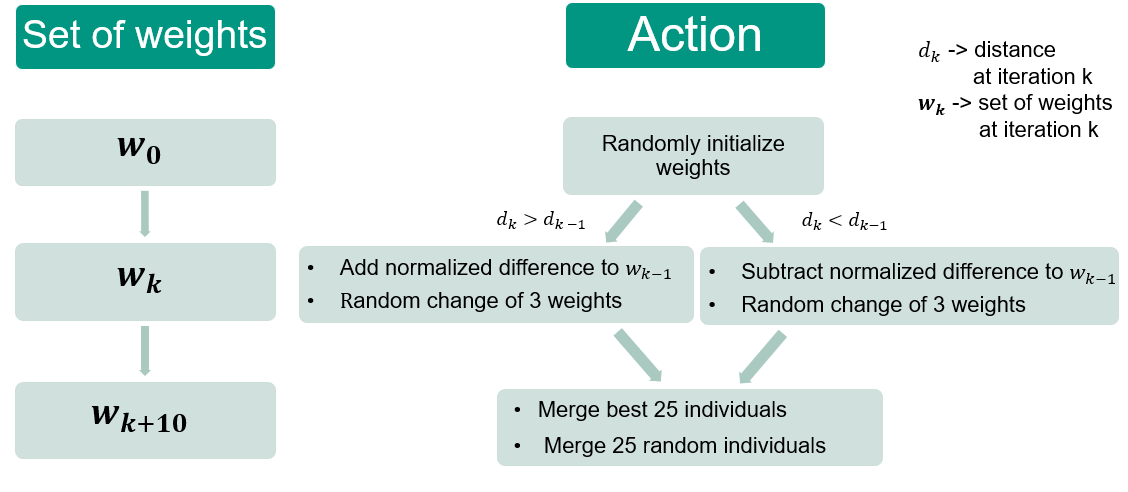
\includegraphics[width=3.3in]{img/evo_strat_1.png}
	\DeclareGraphicsExtensions.
	\caption{Overview of the implementation of the evolutionary algorithm 1}
	\label{fig:evo_strat_1}
\end{figure}

\subsubsection{Evolutionary Strategy 2}
\label{sec:strategie_2}
The second mutation algorithm we evaluated for learning the synaptic weights of the network is based on the evolutionary strategy introduced by Salimans et al. \cite{Salimans2017EvolutionSA}. Their algorithm repeatedly executes two phases 1) Random Perturbation of the weights and evaluation the resulting parameters by running the experiment and the 2) Combining the results of the individual perturbations to compute an estimation for the stochastic gradient decent to update the weights. The algorithm is shown below: 
\begin{algorithm}
	\caption{Evolutionary Strategy 2}
	\begin{algorithmic}[1]
		\renewcommand{\algorithmicrequire}{\textbf{Input:}}
		\REQUIRE Learning rate $\alpha$, noise standard deviation $\sigma$, initial weights $w$
		\FOR {$t = 0,1,2, ...$}
		\STATE Sample $\epsilon_{1},...,\epsilon_{n} \sim \mathcal{N}\left( 0, I \right)$
		\STATE Compute $F_{ i } = F(w_{ i } + \sigma \epsilon_{ i }= for i = 1, ..., n$
		\STATE Set $w_{ t+1 } \leftarrow  w_{ t }+ \alpha \frac{ 1 }{ n \sigma } \sum_{ j = 1 }^{ n }{F_{ j } \epsilon_{ j }  }$
		\ENDFOR
	\end{algorithmic} 
\end{algorithm}

Since the simulation in our experiment is non deterministic it should provide more stable results that the local region of an individual is evaluated more closely, before the synaptic weights are updated.
